\chapter{Projektvorschlag}
\thispagestyle{fancy}
\section{Ausgangssituation}
Zusammenarbeit im Hinblick auf gemeinsames Bearbeiten von Dateien findet bei Projektmitgliedern, die örtlich getrennt sind, oft durch Austausch der Dokumente per Email statt. Dies bedeutet umfangreiche Mailarchive mit vielfacher Speicherung der Dateien. Die Verwaltung von Dateien unterschiedlicher Versionen wird oft durch simple Kopien gelöst. 

In Software-Projekten werden zentrale SCM (Source Code Management)-Server verwendet, über die hauptsächlich Text-Dateien versioniert werden. Dies ist in anderen Branchen eher untypisch. Der SCM-Server muss vom Internet erreichbar sein und verlangt technische Kenntnisse. Ist der zentrale Server nicht unter eigener Verwaltung, besteht ein Datensicherheitsrisiko.

Einige Webportale bieten derzeit die kollaborative Bearbeitung von Officedokumenten in Echtzeit an. Dies ist aber oft auf ein Dokument beschränkt oder nicht als mittelfristige Dateiverwaltung geeignet.

Existierende Kollaborationslösungen sind oft auf eine Plattform oder sogar nur auf ein Dateisystem beschränkt, oder erlauben nur das Bearbeiten von Dokumenten einer Office-Suite.

In kleineren Projekten werden Ankündigungen meist per Mail an alle Teilnehmer versandt, was schnell unübersichtlich werden kann und meist auch nicht explizit archiviert wird.

\section{Projektbeschreibung}
Dieses Projekt soll den Grundstein für eine Plattform legen, die es erlaubt, über ein Netzwerk (z.B. das Internet) gemeinsam an Dateien beliebigen Formats zu arbeiten. Es soll ein Fat Client entwickelt werden, der alle Funktionen der Synchronisationsschnittstelle benutzt, die Implementierung der Netzwerk- und Synchronisationsservices ist aber erst in darauf folgenden Ausbauphasen in Form eigenständiger Projekte geplant. Änderungen an Dateien sollen vom Programm erkannt werden und mit Hilfe der Synchronisations- und Netzwerkservices an andere User propagiert werden. In diesem Projekt soll nur die unten beschrieben Phase 1 realisiert werden.

\section{Zielgruppe/Scope}
Personen, die geringe bis mittlere Computererfahrung haben und in Projekten Dateien verschiedener Formate austauschen und zusammen bearbeiten möchten. 

\subsubsection{Modellszenario}
Eine Projektgruppe, deren 3-12 Mitglieder auf verschiedenen Rechnern arbeiten, die vorwiegend online sind und gemeinsam 5-100 Dateien benutzen. Eine einzelne Datei wird dabei meist nur gleichzeitig von einem Benutzer bearbeitet. 

Dieses Modellszenario könnte in kleinere Firmenprojekten oder in studentischen Projekten (eventuell neben einem SCM) Anwendung finden. Etwa Architekten, die in Projektordnern Formate wie Autocad und Word-Dokumente verwenden, aber in verschiedenen Standorten, z.B. Wien und Abu Dhabi verteilt sind. 

\section{Eingrenzung/Phased Release}

\subsection{Phase 1, Fat Client}
In dieser Phase wird das Programm als Fat Client erstellt, dessen grafischen Oberfläche die vollständige Nutzbarkeit der unten aufgeführten Features benutzbar macht. 
Die Netzwerkkommunikation zwischen verschiedenen Clients soll mithilfe eines Mock-Service simuliert werden. Dieser Service wird in dieser Phase die Zusammenarbeit mit anderen Clients simulieren, wodurch die Funktionalität des Programmes getestet werden kann. Neben diesem Mock-Service, welches die Netzwerkservices der Anwendung kapselt, wird zusätzlich noch ein Synchronisationsinterface erstellt, welches es erlaubt, den Vorgang der Synchronisation zwischen den Clients, auf verschiedene Weisen zu implementieren.
Die Synchronisation soll in dieser Phase ebenfalls mithilfe eines Mock-Services  realisiert werden. Die Netzwerk- und Synchronisations-Mock-Services können dann in möglichen späteren Projektphasen durch entsprechende Implementierungen (z.B. XMPP für das Netzwerkservice) ersetzt werden. Die für die Synchronisation notwendigen Elemente der Benutzeroberfläche sollen aber bereits in dieser Phase erstellt und an die entsprechenden Schnittstellen gebunden werden. 

\subsubsection{Aufgaben des Networkservice}
Authentifizierung der Benutzer
Netzwerkverbindung zwischen den Clients
Austausch von Nachrichtenpaketen zwischen den Clients
Datenaustausch zwischen den Clients

\subsubsection{Aufgaben des Synchronisationsservice}
Abholen von Dateiversionen, die andere Projektmitglieder erstellt haben
Verbreiten eigener Änderungen
Abgleich von Dateiversionen zwischen Clients
Erkennen von Dateikonflikten
\subsection{Phase 2, Networking / Synchronisation}
Die Mock-Services werden durch konkrete  Implementierungen des Networkservice und des Synchronisationsservice ersetzt. Für das Networkservice ist zur Zeit eine Lösung auf Basis des XMPP-Protokolles angedacht. Durch eine generischen Definition der Schnittstellen in Phase 1 kann dies aber auch mit beliebigen anderen Technologien erfolgen.
\subsection{Phase 3, Service Sharing}
In dieser Phase ist das zur Verfügung stellen lokaler Services (z.B. Printer Server) zwischen den Projektmitgliedern geplant.

\section{Featureliste}

\begin{tabular}{ | c | p{10.5cm} | c |}
\hline
\textbf{Phase} & \textbf{Beschreibung} & \textbf{}\\
\hline
1 & Netzwerkservice wird durch generische Schnittstelle definiert und als Mock-Service implementiert & Muss\\
\hline
1 & Synchronisationsalgorithmus wird durch generische Schnittstelle definiert und als Mock-Service implementiert & Muss\\
\hline
1 & Verwaltung der Mitglieder des Projektes & Muss\\
\hline
1 & Dateien beliebigen Formats und Notizen können Metadaten angehängt werden & Muss\\
\hline
1 & Verwaltung (hinzufügen, bearbeiten, entfernen) der Dateien und Notizen & Muss\\
\hline
1 & Alle für die Konfliktbehandlung notwendigen Benutzerelemente sind verfügbar & Muss\\
\hline
1 & Dateien können offline bearbeitet werden & Muss\\
\hline
1 & Dateien sind im Dateisystem, ohne die Applikation verwenden zu müssen, verfügbar & Soll\\
\hline
1 & Änderungen der Dateien im Dateisystem werden vom Programm erkannt und propagiert & Muss\\
\hline
1 & Dateien und Notizen in Kategorien eingeteilt werden und es können & Muss\\
\hline
1 & Dateien und Notizen können aufgrund der Tags gesucht bzw. aufgelistet werden & Muss\\
\hline
2 & Implementierung des Netzwerkservice mittels z.B. XMPP & Muss\\
\hline
2 & Implementierung einer Synchronisationsstrategie & Muss\\
\hline
3 & Projektmitglieder können Netzwerkdienste, die für sie verfügbar sind, anderen freigeben, die sie dann mitbenutzen können. & Muss\\
\hline
3 & Es ist ersichtlich, wer welche Dienste freigibt und wer die freigegeben Dienste im Moment mitbenutzt. & Muss\\
\hline
\end{tabular} 

\section{Domänenmodell}
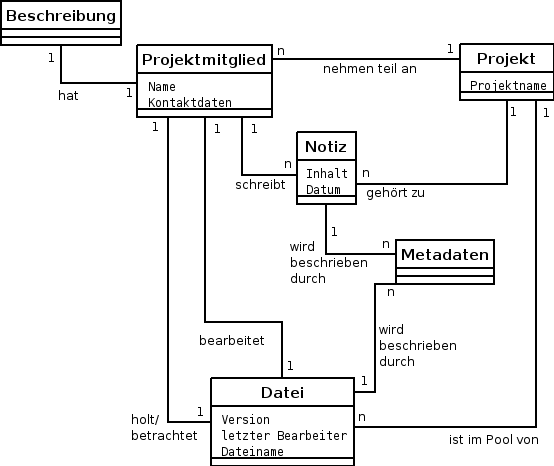
\includegraphics[width=0.97\textwidth]{../uml/domain_model.png}
